
\documentclass[12pt]{report}

\usepackage{fullpage}
\usepackage{graphicx}
\usepackage{listings}
\usepackage{verbatim}
\usepackage{amsmath}
\usepackage{color}
\usepackage{hyperref}
 
\definecolor{codegreen}{rgb}{0,0.6,0}
\definecolor{codegray}{rgb}{0.5,0.5,0.5}
\definecolor{codepurple}{rgb}{0.58,0,0.82}
\definecolor{backcolour}{rgb}{0.95,0.95,0.92}
 
\lstdefinestyle{mystyle}{
    backgroundcolor=\color{backcolour},   
    commentstyle=\color{codegreen},
    keywordstyle=\color{magenta},
    numberstyle=\tiny\color{codegray},
    stringstyle=\color{codepurple},
    basicstyle=\footnotesize,
    breakatwhitespace=false,         
    breaklines=true,                 
    captionpos=b,                    
    keepspaces=true,                 
    numbers=left,                    
    numbersep=5pt,                  
    showspaces=false,                
    showstringspaces=false,
    showtabs=false,                  
    tabsize=2
}
 
\lstset{style=mystyle}
\renewcommand{\baselinestretch}{2}
\author{Mohammed Nauman Sididque}
\title{Assignment 2 }

\begin{document}
\maketitle
\tableofcontents
\chapter{Problem 4.1}
\section{Problem Statement}
Plot rank-frequency curves (using a log-log graph) for words and bigrams in the Wikipedia collection available through the book website (http://www.searchengines-book.com). Plot a curve for the combination of the two. What are the best values for the parameter c for each curve?
\subsection{Rank-Frequency Curve}

Unigrams in the Wikipedia Small Corpus: 225,744\\
Bigrams in the Wikipedia Small Corpus: 1,429,162\\

The reason for the graphs to not converge to the Zipf's Law is due to confined corpus size. The value of constant as 1.2 does not allow the curve for unigrams and bigrams to follow the Zipf's Law trajectory. But in case of constant 0.8, the bigrams follow the Zipf's Law tajectory in the middle of their curve.

The graph used to plot the graph is :

\[log cf_i = log c + k log i\] where k=-1, c is a constant and f is frequency of the word with rank i

The graph with unigram and bigram distribution for constant value of 1.2 is shown in figure. 1.1.  

\begin{figure}[ht] 
  \centering
  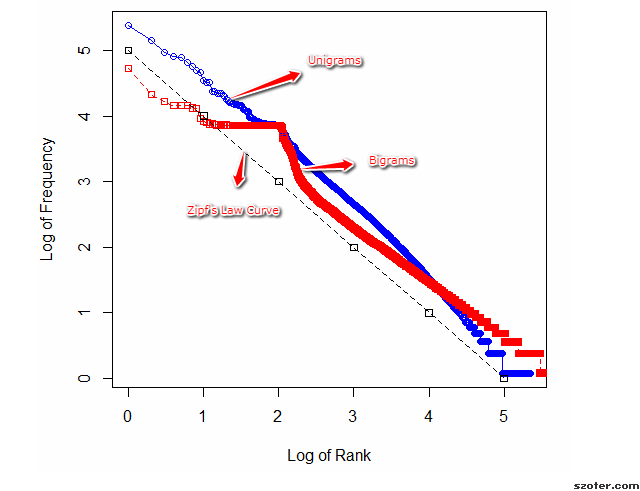
\includegraphics[width=0.7\textwidth]{Problem41.png}
  \caption{ rank-frequency curve (c= 1.2)}
  \label{fig:1}
\end{figure}

The graph with unigram and bigram distribution for constant value of 0.8 is shown in figure.1.2
 
\begin{figure}[ht] 
  \centering
  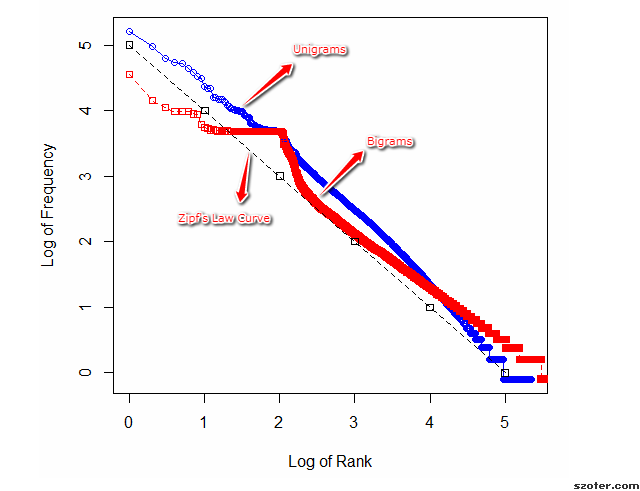
\includegraphics[width=0.7\textwidth]{Problem41C08.png}
  \caption{ rank-frequency curve (c= 0.8)}
  \label{fig:2}
\end{figure}

\chapter{Problem 4.2}
\section{Problem Statement}
Plot vocabulary growth for the Wikipedia collection and estimate the parameters for Heaps’ law. Should the order in which the documents are processed make any difference?
\subsection{Heap's Law Curve}

Monograms in the Wikipedia Small Corpus: 225,744
Total Vocabulary in the Wikipedia Small Corpus: 3,902,115


\chapter{Problem 4.3}
\section{Problem Statement}
Try to estimate the number of web pages indexed by two different search engines using the technique described in this chapter. Compare the size estimates from a range of queries and discuss the consistency (or lack of it) of these estimates. 
\section{Independent Query}
\subsection{Bing Results}
\subsubsection{Query: Dog Mumbai}
For Query, Dog: 228,000,000\\
For Query, Mumbai: 89,000,000\\
For Query, Dog Mumbai: 19,100,000\\

Total collection size = 1,062,000,000\\

\begin{figure}[ht] 
  \centering
  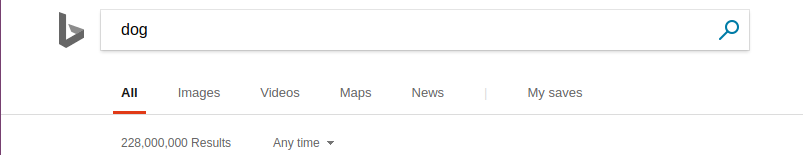
\includegraphics[width=0.7\textwidth]{Bing_Dog.png}
  \caption{Bing Results for Dog}
  \label{fig:1}
\end{figure}

\begin{figure}[ht] 
  \centering
  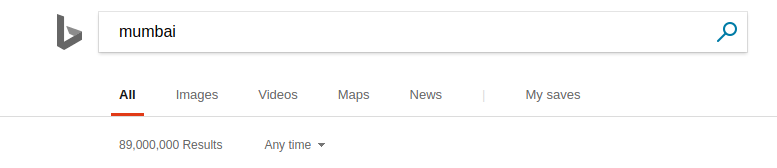
\includegraphics[width=0.7\textwidth]{Bing_Mumbai.png}
  \caption{Bing Results for Mumbai}
  \label{fig:2}
\end{figure}

\begin{figure}[ht] 
  \centering
  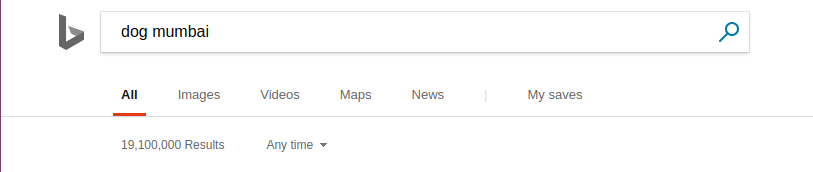
\includegraphics[width=0.7\textwidth]{Bing_dogmumbai.png}
  \caption{Bing Results for Dog Mumbai}
  \label{fig:3}
\end{figure}

\subsubsection{Query:Norfolk Nauman}
For Query, Norfolk: 124,000,000\\
For Query, Nauman: 3,820,000\\
For Query, Norfolk Nauman: 357,000\\

Total collection size = 3,249,000,000\\

\begin{figure}[ht] 
  \centering
  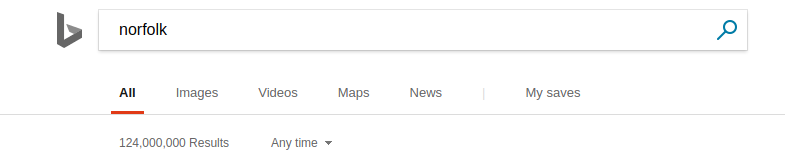
\includegraphics[width=0.7\textwidth]{Bing_norfolk.png}
  \caption{Bing Results for Norfolk}
  \label{fig:4}
\end{figure}

\begin{figure}[ht] 
  \centering
  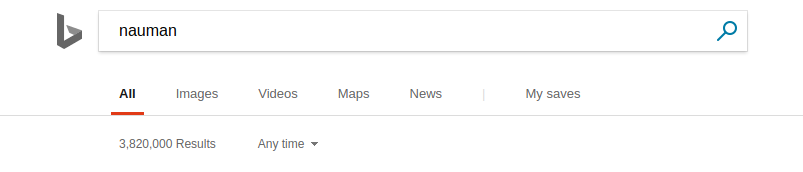
\includegraphics[width=0.7\textwidth]{Bing_nauman.png}
  \caption{Bing Results for Nauman}
  \label{fig:5}
\end{figure}

\begin{figure}[ht] 
  \centering
  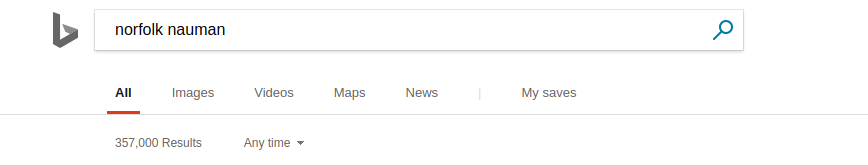
\includegraphics[width=0.7\textwidth]{Bing_norfolknauman.png}
  \caption{Bing Results for Norfolk Nauman}
  \label{fig:6}
\end{figure}

\subsection{Google Results}
\subsubsection{Query: Dog Mumbai}
For Query, Dog: 1,900,000,000\\
For Query, Mumbai: 391,000,000\\
For Query, Dog Mumbai: 17,000,000\\

Total collection size = 43,700,000,000

\begin{figure}[ht] 
  \centering
  
\includegraphics[width=0.7\textwidth]{Google_Dog.png}
  \caption{Google Results for Dog}
  \label{fig:7}
\end{figure}

\begin{figure}[ht] 
  \centering
  
\includegraphics[width=0.7\textwidth]{Google_mumbai.png}
  \caption{google Results for Mumbai}
  \label{fig:8}
\end{figure}

\begin{figure}[ht] 
  \centering
  
\includegraphics[width=0.7\textwidth]{Google_dogmumbai.png}
  \caption{Google Results for Dog Mumbai}
  \label{fig:9}
\end{figure}

\subsubsection{Query:Norfolk Nauman}
For Query, Norfolk: 278,000,000\\
For Query, Nauman: 3,880,000\\
For Query, Norfolk Nauman: 332,000\\

Total collection size = 3,249,000,000\\

\begin{figure}[ht] 
  \centering
  \includegraphics[width=0.7\textwidth]{Google_norfolk.png}
  \caption{Google Results for Norfolk}
  \label{fig:10}
\end{figure}

\begin{figure}[ht] 
  \centering
  
\includegraphics[width=0.7\textwidth]{Google_nauman.png}
  \caption{Google Results for Nauman}
  \label{fig:11}
\end{figure}

\begin{figure}[ht] 
  \centering
  
\includegraphics[width=0.7\textwidth]{Google_norfolknauman.png}
  \caption{Google Results for Norfolk Nauman}
  \label{fig:12}
\end{figure}

\section{Correlated Query}
\subsection{Bing Results}
\subsubsection{Query: Tropical Fish}
For Query, Tropical: 117,000,000\\
For Query, Fish: 175,000,000\\
For Query, Tropical Fish: 19,500,000\\

Total collection size = 1,050,000,000\\

\begin{figure}[ht] 
  \centering
  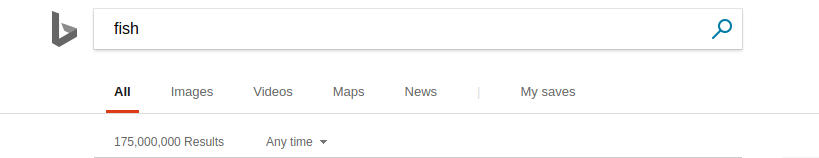
\includegraphics[width=0.7\textwidth]{Bing_Fish.png}
  \caption{Bing Results for Fish}
  \label{fig:13}
\end{figure}

\begin{figure}[ht] 
  \centering
  \includegraphics[width=0.7\textwidth]{Bing_tropical.png}
  \caption{Bing Results for Tropical}
  \label{fig:14}
\end{figure}

\begin{figure}[ht] 
  \centering
  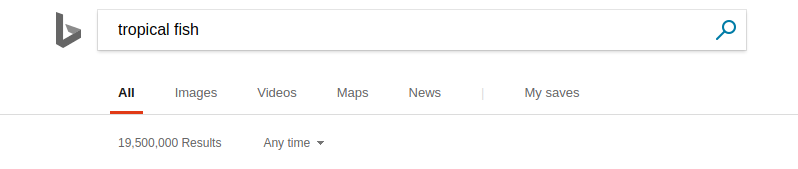
\includegraphics[width=0.7\textwidth]{Bing_tropicalfish.png}
  \caption{Bing Results for Tropical Fish}
  \label{fig:15}
\end{figure}

\subsubsection{Query:Manchester United}
For Query, Manchester: 117,000,000\\
For Query, United: 409,000,000\\
For Query, Manchester United: 6,540,000\\

Total collection size = 7,310,000,000\\

\begin{figure}[ht] 
  \centering
  
\includegraphics[width=0.7\textwidth]{Bing_manchester.png}
  \caption{Bing Results for Manchester}
  \label{fig:16}
\end{figure}

\begin{figure}[ht] 
  \centering
  
\includegraphics[width=0.7\textwidth]{Bing_united.png}
  \caption{Bing Results for United}
  \label{fig:17}
\end{figure}

\begin{figure}[ht] 
  \centering
  
\includegraphics[width=0.7\textwidth]{Bing_manchesterunited.png}
  \caption{Bing Results for Manchester United}
  \label{fig:18}
\end{figure}

\subsection{Google Results}
\subsubsection{Query: Tropical Fish}
For Query, Tropical: 571,000,000\\
For Query, Fish: 1,180,000,000\\
For Query, Tropical Fish: 137,000,000\\

Total collection size = 4,920,000,000\\

\begin{figure}[ht] 
  \centering
  
\includegraphics[width=0.7\textwidth]{Google_fish.png}
  \caption{Google Results for Fish}
  \label{fig:19}
\end{figure}

\begin{figure}[ht] 
  \centering
  \includegraphics[width=0.7\textwidth]{Google_tropical.png}
  \caption{Google Results for Tropical}
  \label{fig:20}
\end{figure}

\begin{figure}[ht] 
  \centering
  \includegraphics[width=0.7\textwidth]{Google_tropicalfish.png}
  \caption{Google Results for Tropical Fish}
  \label{fig:21}
\end{figure}

\subsubsection{Query:Manchester United}
For Query, Manchester: 517,000,000\\
For Query, United: 4,840,000,000\\
For Query, Manchester United: 145,000,000\\

Total collection size = 172,700,000,000\\


\begin{figure}[ht] 
  \centering
  \includegraphics[width=0.7\textwidth]{Google_manchester.png}
  \caption{Google Results for Manchester}
  \label{fig:22}
\end{figure}

\begin{figure}[ht] 
  \centering
  \includegraphics[width=0.7\textwidth]{Google_united.png}
  \caption{Google Results for United}
  \label{fig:23}
\end{figure}

\begin{figure}[ht] 
  \centering
  
\includegraphics[width=0.7\textwidth]{Google_manchesterunited.png}
  \caption{Google Results for Manchester United}
  \label{fig:24}
\end{figure}

\section{Conclusion}
The formula used to estimate the collection size of a search engine assumes that all the query terms are independent. This assumption is not valid for many query terms which are most likely to be correlated. In the above solution the collection size for Google does not converge to anypoint. It fluctuates by degree of 1, which is not acceptable in estimating the collection size. For Bing the collection size results have a bit convergence but the value of the collection size is very much dependent on the query terms. 

\chapter{Problem 4.8}
\section{Problem Statement}
Find the 10 Wikipedia documents with the most inlinks. Show the collection of anchor text for those pages.
\section{Top 10 Wikipedia Documents with most Inlinks}
The results are based on Wikipedia small dataset.
 Top 10 Documents with most inlinks are:\\
Frequency File Name\\
  12088 index.html\\
  12086 Wikipedia\%7EAbout\_8d82.html\\
   6043 Wikipedia\%7EGeneral\_disclaimer\_3e44.html\\
   6043 Wikipedia\%7EContact\_us\_afd6.html\\
   6043 Wikipedia\%7ECommunity\_Portal\_6a3c.html\\
   6043 Special\%7ERecentChanges\_e0d0.html\\
   6043 Portal\%7EFeatured\_content\_5442.html\\
   6043 Portal\%7ECurrent\_events\_bb60.html\\
   6043 Portal\%7EContents\_b878.html\\
   6043 Help\%7EContents\_22de.html\\

Anchor texts for all the top 10 Documents are:\\

1. Anchor text for Index.html: Main Page\\
2. Anchor text for Wikipedia\%7EAbout\_8d82.html: About Wikipedia\\ 
3. Anchor text for Wikipedia\%7EContact\_us\_afd6.html: Contact Wikipedia\\
4. Anchor text for Wikipedia\%7ECommunity\_Portal\_6a3c.html: Community portal\\
5. Anchor text for Wikipedia\%7EGeneral\_disclaimer\_3e44.html: Disclaimers\\
6. Anchor text for Portal\%7ECurrent\_events\_bb60.html:Current events\\
7. Anchor text for Portal\%7EFeatured\_content\_5442.html: Featured content\\
8. Anchor text for Special\%7ERecentChanges\_e0d0.html: Recent changes\\
9. Anchor text for Portal\%7EContents\_b878.html:Contents\\
10. Anchor text for Help\%7EContents\_22de.html: Help\\

These top 10 documents do not lie in the Wikipedia small dataset. The reason for their large number of links is due to their presence on almost every page. There was total 111 inlinks to the pages in the dataset. The top 10 pages with most inlinks are arranged in increasing order:\\
    Frequency File Name\\
      2 the United States.html\\
      2 township.html\\
      2 townships.html\\
      2 the South Sandwich Islands.html\\
      3 settlements.html\\
      5 Portal.html\\
      8 (at 25 °C, 100 kPa).html\\
      9 states.html\\
     18 community.html\\
     54 communities.html\\

\chapter{Problem 5.14}
\section{Problem Statement}
In section 5.7.3, we saw that the optimal skip distance c can be determined by minimizing the quantity kn/c + pc/2, where k is the skip pointer length, n is the total inverted list size, c is the skip interval, and p is the number of postings to find. Plot this function using k = 4, n = 1,000,000, and p = 1,000, but varying c. Then, plot the same function, but set p = 10,000. Notice how the optimal value for c changes. Finally, take the derivative of the function kn/c + pc/2 in terms of c to find the optimum value for c for a given set of other parameters (k, n, and p).
\section{Optimal Skip Distance}

For value  k = 4, n = 1,000,000, and p = 1,000 and c in [5,50] with step-size of 5. As the value of c increases, the total number of bytes read decreases. With respect to this graph the value of c is too large to be considered for optimal skip distance. The optimal skip distance will lie above 50 in range of approx  60 to 70 for being optimal.  \\
X-axis of graph shows optimal skip distance and Y- axis represents   total number of bytes read.
\begin{figure}[ht] 
  \centering
  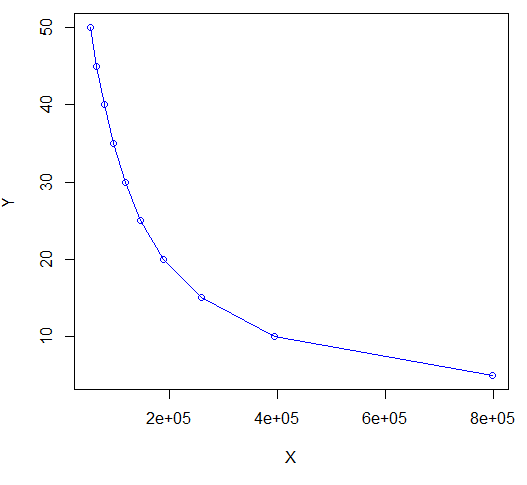
\includegraphics[width=0.7\textwidth]{Case1_514.PNG}
  \caption{Case 1}
  \label{fig:25}
\end{figure}

For value  k = 4, n = 1,000,000, and p = 10,000 and c in [5,50] with step-size of 5. The total number of bytes read decreases below 0 when p is increased from 1,000 to 10,000 for the range of C = {5, 10, 15, 20, 25, 30, 35, 40, 45, 50}. Value of c above approx. 27 is not acceptable for this function, as further increase in c drops the total number of bytes read to a negative number. With respect to this graph c is optimum in range 20 to 25 for optimal skip distance\\

X-axis of graph shows optimal skip distance and Y- axis represents   total number of bytes read.
\begin{figure}[ht] 
  \centering
  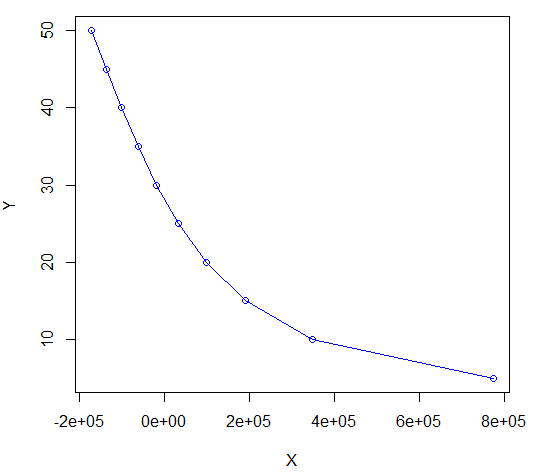
\includegraphics[width=0.7\textwidth]{Case2_514.PNG}
  \caption{Case 2}
  \label{fig:26}
\end{figure}

Differentiating the function: \[kn/c + pc/2\] \\

Results to: \[kn/c^2 + p/2\]

For value =   k = 4, n = 1,000,000, and p = 1,000 and c in [0.5,5] with step-size of 0.5. The total value of  f bytes read decreases.  With respect to this graph c is optimum in around 5 for optimal skip distance\\

X-axis of graph shows optimal skip distance and Y- axis represents   total number of bytes read.
\begin{figure}[ht] 
  \centering
  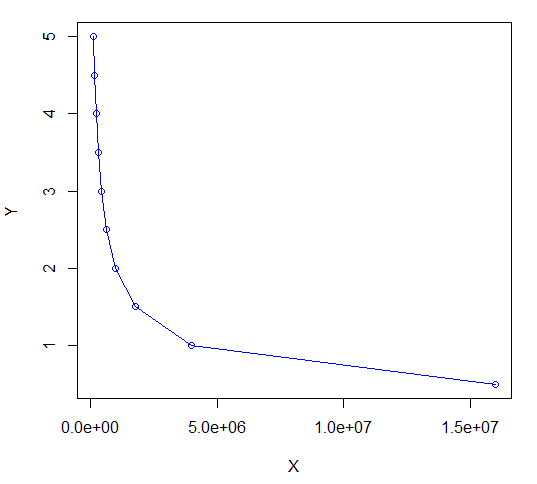
\includegraphics[width=0.7\textwidth]{Case3_514.PNG}
  \caption{Case 3}
  \label{fig:27}
\end{figure}
\end{document}